\documentclass[10pt,a4paper]{article}
\usepackage[utf8]{inputenc}
\usepackage{amsmath}
\usepackage{amsfonts}
\usepackage{amssymb}
\usepackage{caption}
\usepackage{subcaption}
\usepackage{graphicx}
\usepackage[left=2cm,right=2cm,top=2cm,bottom=2cm]{geometry}
\begin{document}
\section*{Subfigure Demo} 
\begin{figure}[h]
 \centering
 \begin{subfigure}[b]{0.3\textwidth}
 \centering
 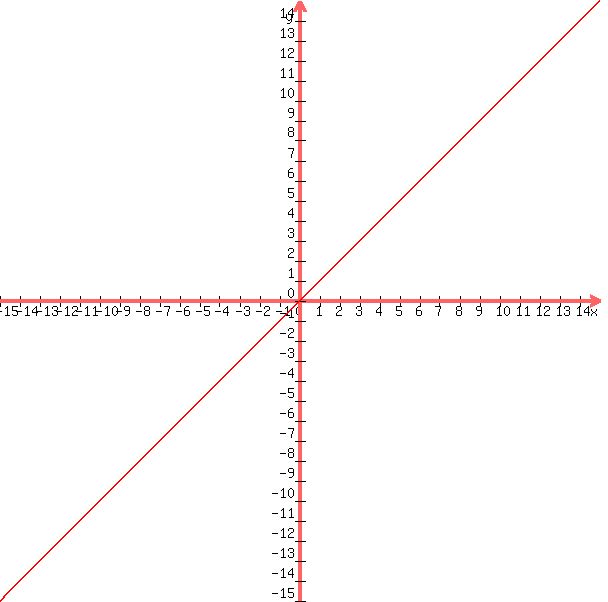
\includegraphics[width=\textwidth]{y=x.jpg} 
 \caption{$y=x$}
 \label{fig:y equals x}
 \end{subfigure}
 \hfill
 \begin{subfigure}[b]{0.3\textwidth}
 \centering
 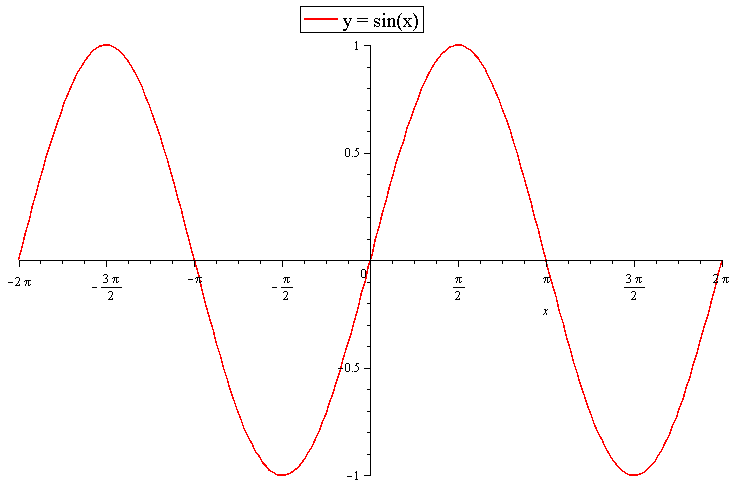
\includegraphics[width=\textwidth]{y=3sinx.jpg}
 \caption{$y=3\sin x$}
 \label{fig:three sin x}
 \end{subfigure}
 \hfill
 \begin{subfigure}[b]{0.3\textwidth}
 \centering
 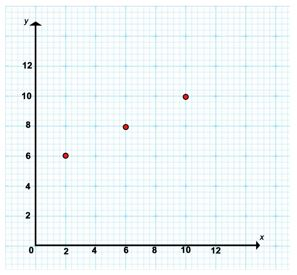
\includegraphics[width=\textwidth]{5divides.jpg}
 \caption{$y=5/x$}
 \label{fig:five over x}
 \end{subfigure}
 \caption{Three simple graphs arranged side-by-side}
 \label{fig:three graphs}
\end{figure}
\end{document}
